\documentclass[hyperref={bookmarks=false},aspectratio=169]{beamer}
\usepackage{hyperref,ragged2e,amsmath,amssymb,url,bm}
\usepackage{graphicx,booktabs,array}
\usepackage{tikz}
\usetikzlibrary{arrows.meta,positioning,calc,shapes.geometric,decorations.pathreplacing,matrix}
\graphicspath{{crops/}}
\usetheme{Goettingen}
% --- Paleta "Israel": café ladrillo (ladrillos de Egipto, Éx 1:14), oro del santuario, piedra de Jerusalén ---
\definecolor{cafe}{RGB}{96,52,30}
\definecolor{cafeosc}{RGB}{50,25,13}
\definecolor{tinta}{RGB}{44,28,18}
\definecolor{oro}{RGB}{196,148,40}
\definecolor{ladrillo}{RGB}{158,70,40}
\definecolor{piedra}{RGB}{240,228,203}
\definecolor{sepia}{RGB}{104,86,62}
\setbeamercolor{structure}{fg=ladrillo}
\setbeamertemplate{sidebar canvas right}[vertical shading][top=ladrillo!92!black,bottom=cafeosc]
\setbeamercolor{title in sidebar}{fg=oro}
\setbeamercolor{author in sidebar}{fg=piedra}
\setbeamercolor{section in sidebar}{fg=piedra}
\setbeamercolor{section in sidebar shaded}{fg=oro!60!piedra!70!cafe}
\setbeamercolor{subsection in sidebar}{fg=piedra}
\setbeamercolor{subsection in sidebar shaded}{fg=oro!60!piedra!70!cafe}
\let\raggedright\justifying
\setbeamertemplate{background canvas}{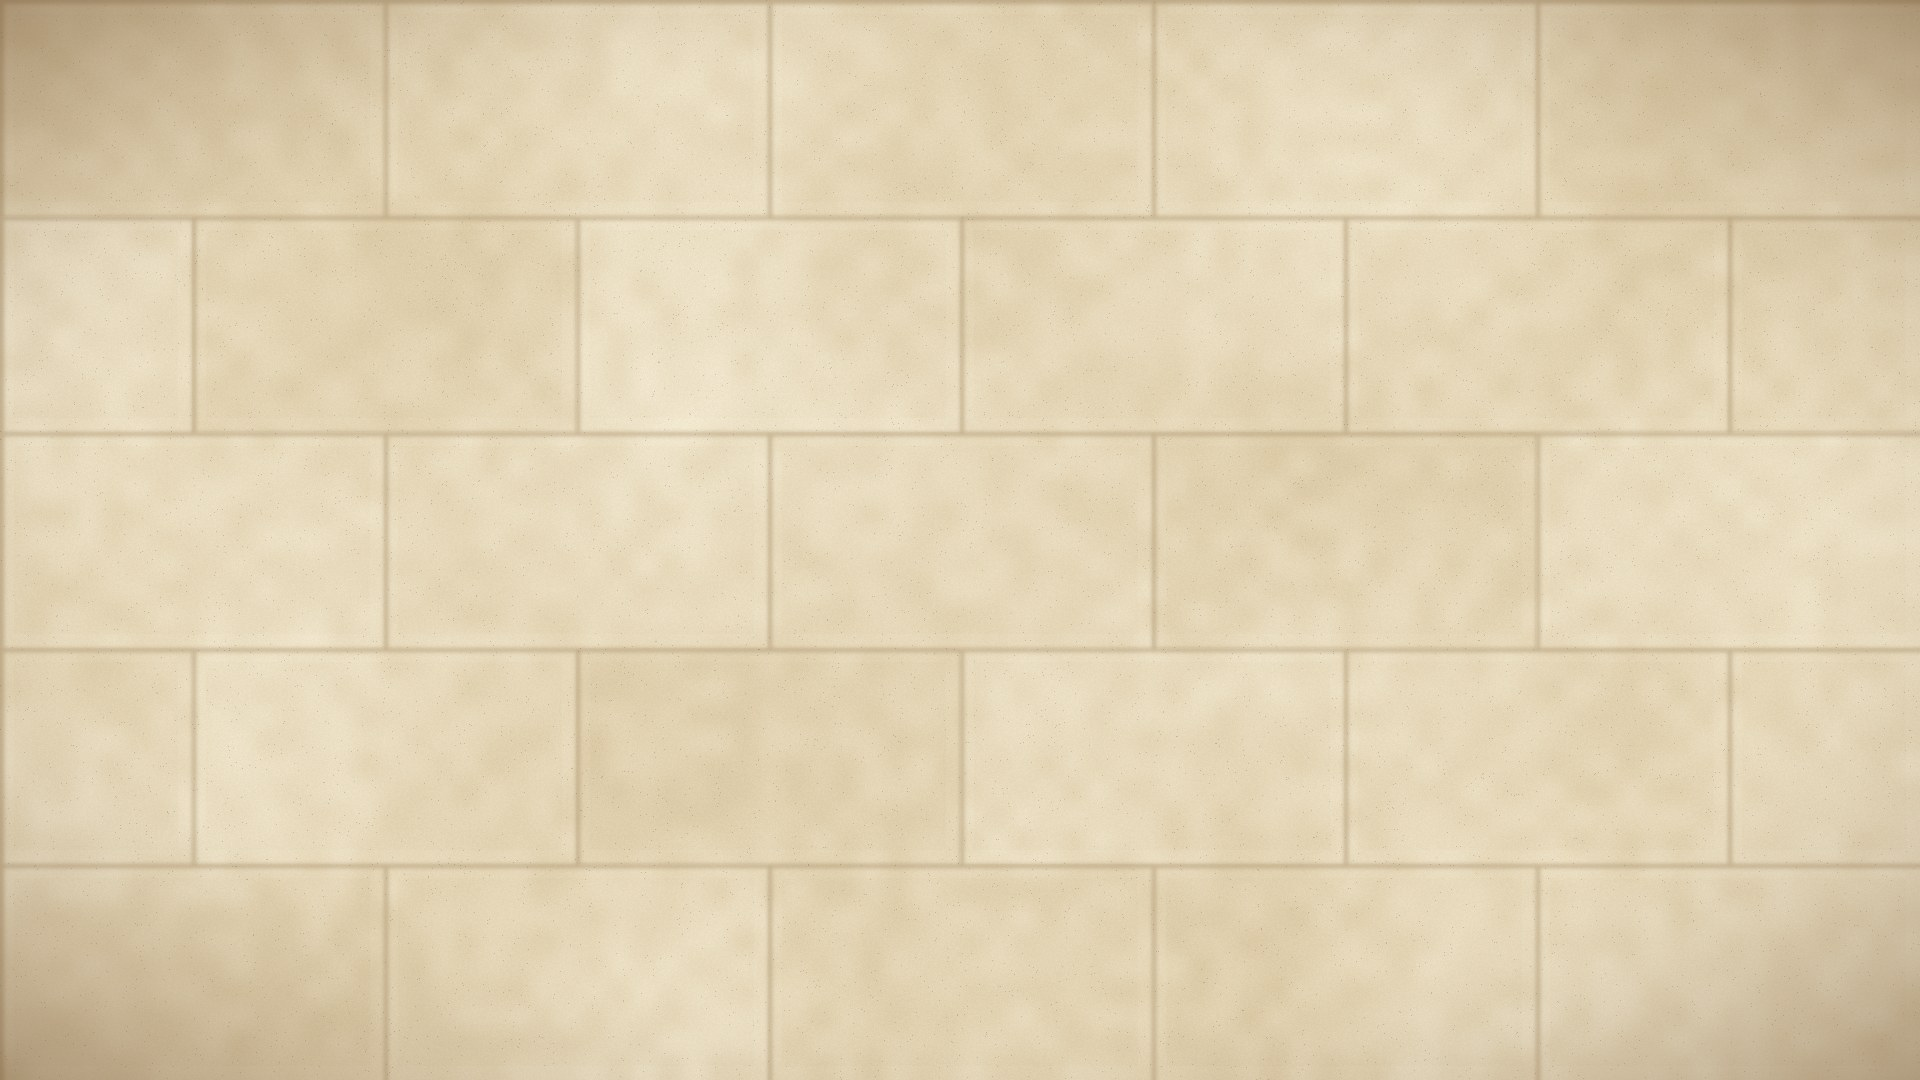
\includegraphics[width=\paperwidth,height=\paperheight]{piedra.jpg}}
\setbeamercolor{normal text}{fg=tinta}
\setbeamercolor{frametitle}{fg=ladrillo}
\setbeamerfont{frametitle}{series=\bfseries}
\setbeamertemplate{section in toc shaded}{\leavevmode{\color{sepia!85!black}\inserttocsection}\par}
\setbeamercolor{title}{fg=ladrillo}
\setbeamercolor{subtitle}{fg=cafe}
\setbeamercolor{item projected}{bg=cafe,fg=piedra}
\setbeamertemplate{itemize item}{\small\textcolor{oro!85!ladrillo}{$\blacktriangleright$}}
\setbeamertemplate{navigation symbols}{}
% --- Español + hebreo + griego (XeLaTeX) con fuentes empaquetadas en fonts/ ---
\usepackage[bidi=default]{babel}
\babelprovide[import,main]{spanish}
\babelprovide[import]{hebrew}
\babelprovide[import]{ancientgreek}
\babelfont[hebrew]{sf}[Path=fonts/, BoldFont=NotoHebrewSans-700.ttf]{NotoHebrewSans-400.ttf}
\babelfont[hebrew]{rm}[Path=fonts/, BoldFont=NotoHebrewSans-700.ttf]{NotoHebrewSans-400.ttf}
\babelfont[ancientgreek]{sf}[Path=fonts/]{GFSPorson.otf}
\babelfont[ancientgreek]{rm}[Path=fonts/]{GFSPorson.otf}
\newcommand{\heb}[1]{\mbox{\foreignlanguage{hebrew}{#1}}}
\newcommand{\grc}[1]{\foreignlanguage{ancientgreek}{#1}}
% --- Citas, imágenes, referencias ---
\usepackage[most]{tcolorbox}
\newtcolorbox{cita}[1][]{enhanced, colback=piedra!92!white, colframe=ladrillo!85!oro,
  boxrule=0pt, leftrule=2.5pt, arc=0pt, left=6pt, right=6pt, top=4pt, bottom=4pt,
  before skip=4pt, after skip=6pt, fontupper=\small\itshape, #1}
\newcommand{\fuente}[1]{\par\hfill{\upshape\bfseries\footnotesize\textcolor{ladrillo}{#1}}}
\newcommand{\imagen}[3][0.80]{%
  \centering\includegraphics[height=#1\textheight,width=\linewidth,keepaspectratio]{#2}\par\vspace{2pt}
  {\fontsize{5}{6}\selectfont\color{sepia}{\raggedleft\textit{Nota.} #3\par}}}
\makeatletter
\newcommand{\fotolado}[2]{%
  \begin{tikzpicture}[remember picture,overlay]
    \node[anchor=north east,inner sep=0pt] (foto) at ([xshift=-\beamer@sidebarwidth]current page.north east)
      {\includegraphics[height=\paperheight]{#1}};
    \node[anchor=south east,inner sep=2pt,text=piedra,fill=cafeosc,fill opacity=0.6,text opacity=1,
      font=\fontsize{4.5}{5.5}\selectfont,align=right,text width=4.2cm] at ([xshift=-3pt,yshift=3pt]foto.south east)
      {\textit{Nota.} #2};
  \end{tikzpicture}}
\makeatother
\newcommand{\refapa}[1]{\par\hangindent=1.2em\hangafter=1\noindent #1\par\vspace{3pt}}
\usepackage{xurl}\urlstyle{same}
\newcommand{\destacar}[1]{\textbf{\textcolor{ladrillo}{#1}}}
\usetikzlibrary{shadows}
\tikzset{caja/.style={draw=cafe!80!black,line width=0.7pt,top color=piedra!55!white,bottom color=piedra!92!oro,
  rounded corners=4pt,inner sep=5pt,font=\scriptsize,
  drop shadow={shadow xshift=0.7pt,shadow yshift=-0.8pt,opacity=0.25,fill=cafeosc}},
  >={Stealth[length=2.4mm,width=1.8mm]}, every picture/.style={line cap=round,line join=round}}
\newcommand{\precision}[1]{{\footnotesize\color{sepia}\textbf{Precisión:} #1}}
\newcommand{\pt}[2]{({#1-30},{#2-29})}
\title[Israel 4: David--división]{\bfseries{Israel, el pueblo de Dios}}
\subtitle{Estudio 4. De David a la división del reino}
\author{}\institute{}\date{}
\titlegraphic{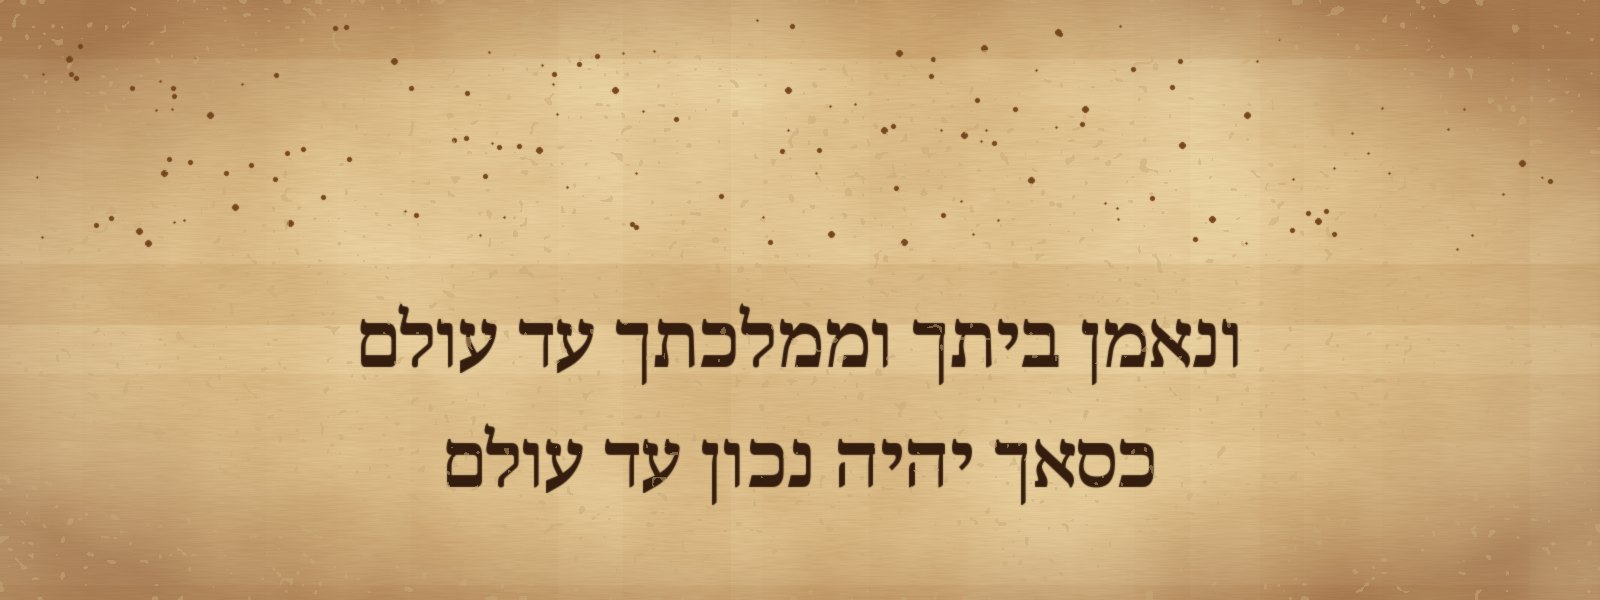
\includegraphics[width=0.85\linewidth,height=0.38\textheight,keepaspectratio]{portada.jpg}\\[-1pt]
  {\fontsize{5}{6}\selectfont\color{sepia}\textit{Nota.} Elaboración propia: 2~S 7:16 en texto hebreo consonántico (BHS).}}
\AtBeginSection[]{\begin{frame}\frametitle{Contenidos}\tableofcontents[currentsection]\end{frame}}
\begin{document}
\frame{\titlepage}
\begin{frame}\frametitle{Contenidos}\tableofcontents\end{frame}

% ===================================================
\section{Introducción}
\begin{frame}{¿Una promesa «para siempre»?}
\begin{columns}[t,onlytextwidth]
\begin{column}{0.52\textwidth}
\begin{cita}Y será firme tu casa y tu reino para siempre delante de ti, y tu trono será estable para siempre.\fuente{(2~S 7:16)}\end{cita}
\begin{cita}¿Qué parte tenemos nosotros con David? [\ldots] ¡Israel, a tus tiendas!\fuente{(1~R 12:16)}\end{cita}
\end{column}
\begin{column}{0.45\textwidth}\small
Menos de un siglo separa la promesa del cisma.\par\medskip
\destacar{Tesis 1.} El pacto davídico concentra la vocación de Éx 19:6 en un rey, una ciudad y una casa de oración «para todos los pueblos» (1~R 8:41--43).\par\medskip
\destacar{Tesis 2.} La división es juicio, pero con límite: Dios aflige a la casa de David «pero no para siempre» (1~R 11:39).
\end{column}
\end{columns}
\end{frame}

\begin{frame}{Los ejes de la serie en esta etapa}
\centering
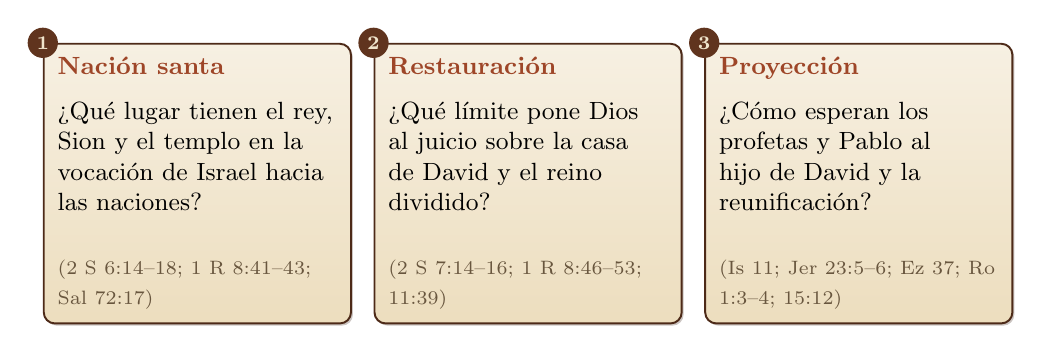
\begin{tikzpicture}
 \foreach \x/\n/\t/\d/\r in {0/1/{Nación santa}/{¿Qué lugar tienen el rey, Sion y el templo en la vocación de Israel hacia las naciones?}/{2~S 6:14--18; 1~R 8:41--43; Sal 72:17},
   4.2/2/{Restauración}/{¿Qué límite pone Dios al juicio sobre la casa de David y el reino dividido?}/{2~S 7:14--16; 1~R 8:46--53; 11:39},
   8.4/3/{Proyección}/{¿Cómo esperan los profetas y Pablo al hijo de David y la reunificación?}/{Is 11; Jer 23:5--6; Ez 37; Ro 1:3--4; 15:12}}{
  \node[caja,anchor=north] (b\n) at (\x,0) {\parbox[t][3.2cm][t]{3.55cm}{\RaggedRight
    {\small\textbf{\textcolor{ladrillo}{\t}}}\\[5pt]\small \d\par\vfill{\scriptsize\color{sepia}(\r)}}};
  \node[circle,fill=cafe,text=piedra,font=\scriptsize\bfseries,inner sep=1.6pt] at (b\n.north west) {\n};}
\end{tikzpicture}\par\vspace{6pt}
{\scriptsize\color{sepia}Las citas bíblicas son traducción propia desde el texto hebreo (BHS) y griego (NA28). Numeración española [hebrea] cuando difiere.}
\end{frame}

\begin{frame}{Tres sentidos de «Israel»}
\centering\scriptsize\renewcommand{\arraystretch}{1.25}
\begin{tabular}{>{\RaggedRight\arraybackslash}p{2.2cm}>{\RaggedRight\arraybackslash}p{5.0cm}>{\RaggedRight\arraybackslash}p{3.6cm}}
\toprule
\textbf{Sentido} & \textbf{Referente} & \textbf{Ejemplos}\\\midrule
\textbf{Israel} (pueblo) & Las doce tribus, descendencia de Jacob & 2~S 7:10; 1~R 8:62; Ro 11:1\\
\textbf{Israel} (norte) & Diez tribus, centro en Efraín; capitales Siquem, Penuel, Tirsa y, desde Omri, Samaria & 2~S 2:9; 1~R 12:16--20; Os 5:3\\
\textbf{Judá} (sur) & Judá y Benjamín; Jerusalén; casa de David & 2~S 2:4; 1~R 12:21\\
\bottomrule
\end{tabular}\par\vspace{8pt}
\begin{minipage}{0.92\linewidth}\small
\destacar{«Todo Israel»} no siempre es el pueblo entero: en 1~R 8:62 son todas las tribus; en 1~R 12:16--20, solo las del norte. Aun en el reino unido el texto dice «Israel y Judá» (2~S 5:5; 1~R 4:20).\par\smallskip
\precision{la pregunta vuelve en Ro 11:26, «todo Israel será salvo» (Estudio 8).}
\end{minipage}
\end{frame}

\begin{frame}{Secuencia de la etapa}
\centering
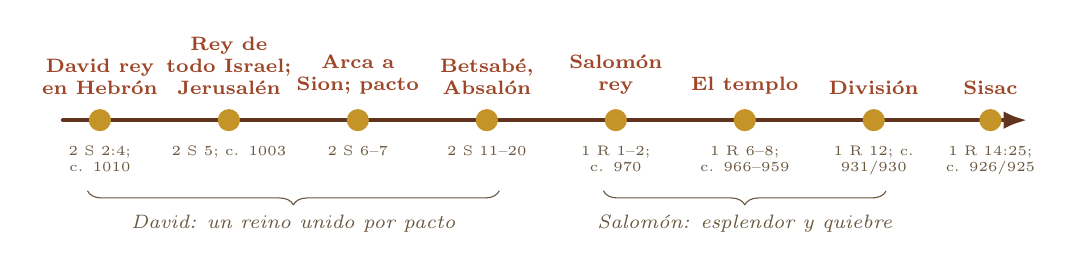
\begin{tikzpicture}[x=0.78cm]
\draw[line width=1.6pt,cafe,-{Latex[length=3mm]}] (0,0) -- (15.7,0);
\foreach \x/\t/\b in {0.6/{David rey en Hebrón}/{2~S 2:4; c. 1010},
                      2.7/{Rey de todo Israel; Jerusalén}/{2~S 5; c. 1003},
                      4.8/{Arca a Sion; pacto}/{2~S 6--7},
                      6.9/{Betsabé, Absalón}/{2~S 11--20},
                      9.0/{Salomón rey}/{1~R 1--2; c. 970},
                      11.1/{El templo}/{1~R 6--8; c. 966--959},
                      13.2/{División}/{1~R 12; c. 931/930},
                      15.1/{Sisac}/{1~R 14:25; c. 926/925}}{
  \fill[oro] (\x,0) circle (4pt);
  \node[above,font=\scriptsize\bfseries,text=ladrillo,text width=1.6cm,align=center] at (\x,0.2) {\t};
  \node[below,font=\tiny,text=sepia,text width=1.6cm,align=center] at (\x,-0.2) {\b};}
\draw[decorate,decoration={brace,amplitude=5pt,mirror},sepia] (0.4,-0.9) -- (7.1,-0.9) node[midway,below=5pt,font=\scriptsize\itshape]{David: un reino unido por pacto};
\draw[decorate,decoration={brace,amplitude=5pt,mirror},sepia] (8.8,-0.9) -- (13.4,-0.9) node[midway,below=5pt,font=\scriptsize\itshape]{Salomón: esplendor y quiebre};
\end{tikzpicture}\par\vspace{4pt}
{\fontsize{5}{6}\selectfont\color{sepia}\raggedleft\textit{Nota.} Elaboración propia. Fechas aproximadas a.\,e.\,c. según Thiele (1983); otras cronologías bajan la división a c. 922.\par}
\end{frame}

\begin{frame}{Fechas y cifras en debate}
\begin{columns}[t,onlytextwidth]
\begin{column}{0.46\textwidth}\small
\textbf{\textcolor{cafe}{La fecha de la división}}
\begin{itemize}
\item \destacar{931/930 a.\,e.\,c.}: Thiele (1983); la usa el material de la Clase 7.
\item \destacar{c. 922 a.\,e.\,c.}: escuela de Albright.
\item Primer sincronismo externo: Sisac, 5.º año de Roboam (1~R 14:25). La lista de Sheshonq~I en Karnak (c. 150 topónimos: Gabaón, Meguido, Négueb) no incluye a Jerusalén en lo legible; golpeó también al norte (Kitchen, 1986).
\end{itemize}
\end{column}
\begin{column}{0.52\textwidth}
\textbf{\small\textcolor{cafe}{¿800.000 en el norte, 400.000 en Judá?}}\par\smallskip
\scriptsize\renewcommand{\arraystretch}{1.2}
\begin{tabular}{>{\RaggedRight\arraybackslash}p{1.9cm}>{\RaggedRight\arraybackslash}p{3.9cm}}
\toprule
\textbf{Fuente} & \textbf{Dato}\\\midrule
2~S 24:9 & Guerreros, no habitantes: 800.000 Israel; 500.000 Judá\\
1~Cr 21:5 & 1.100.000 Israel; 470.000 Judá\\
\emph{Élef} & ¿«mil» o unidad militar? (Mendenhall, 1958)\\
Arqueología & Cientos de miles en todo el territorio en el s. \textsc{viii} (Broshi y Finkelstein, 1992)\\
\bottomrule
\end{tabular}\par\smallskip
\precision{las cifras son estimaciones; se sostiene la proporción: el norte era mayor y más rico.}
\end{column}
\end{columns}
\end{frame}

% ===================================================
\section{Arqueología}
\begin{frame}{Los dos reinos}
\begin{columns}[c,onlytextwidth]
\begin{column}{0.44\textwidth}\centering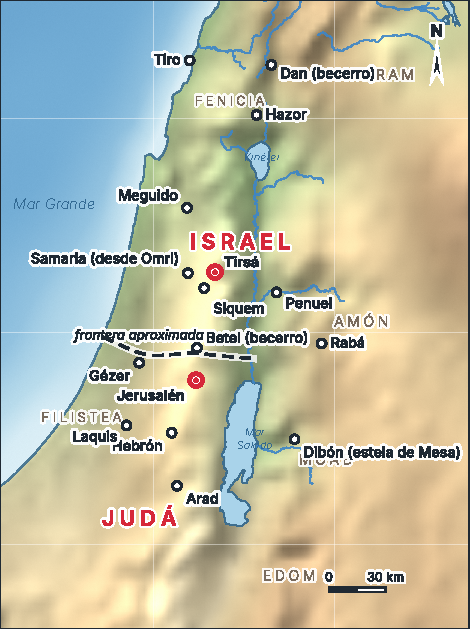
\includegraphics[width=\linewidth,height=0.86\textheight,keepaspectratio]{mapa_division.pdf}\par\vspace{1pt}{\fontsize{4.5}{5.5}\selectfont\color{sepia}\textit{Nota.} Elaboración propia (GSHHS/WDB, Basemap); ubicaciones aproximadas.\par}\end{column}
\begin{column}{0.54\textwidth}\scriptsize\RaggedRight
{\scriptsize\RaggedRight
\makebox[0.6cm][c]{\textcolor{ladrillo}{\rule{0.55ex}{0.55ex}}}~Capital\par
\makebox[0.6cm][c]{\textcolor{cafeosc}{\textbullet}}~Ciudad\par}
\medskip

\textcolor{cafeosc}{\textbf{- - -}} Frontera aproximada: cambió con las guerras (1~R 15:16--22).\par\smallskip
\textbf{Israel (norte)}: más extenso, fértil y poblado; capitales Siquem, Penuel, Tirsá y luego Samaria. Santuarios de Jeroboam en Betel y Dan (1~R 12:29).\par\smallskip
\textbf{Judá (sur)}: montañoso; Jerusalén, en la frontera con Benjamín, y la casa de David.\par\smallskip
Al este, Moab: la estela de Mesa (Dibón) nombra a Omri, rey de Israel.
\end{column}
\end{columns}
\end{frame}

\begin{frame}{La «casa de David» fuera de la Biblia}
\begin{columns}[t,onlytextwidth]
\begin{column}{0.49\textwidth}\small
\textbf{\textcolor{ladrillo}{Estela de Tel Dan}} (c. 840 a.\,e.\,c.)
\begin{itemize}
\item Aramea; Biran, 1993--1994; probablemente Hazael.
\item Mató a [Jo]ram, «rey de Israel» (\heb{מלך ישראל}), y al rey de \heb{ביתדוד}, «casa de David».
\item Primera mención segura de David fuera de la Biblia (Biran y Naveh, 1993, 1995).
\end{itemize}
\precision{un extranjero distingue dos reinos: «Israel» y la «casa de David» (Judá).}
\end{column}
\begin{column}{0.49\textwidth}\small
\textbf{\textcolor{ladrillo}{Estela de Mesa}} (c. 840 a.\,e.\,c.)
\begin{itemize}
\item Moabita; Dibón, 1868. Nombra a «Omri, rey de Israel» y a YHWH.
\item Línea 31: \emph{b[t]dwd} según Lemaire (1994).
\item Finkelstein, Na'aman y Römer (2019): quizá «Balac».
\end{itemize}
\begin{tcolorbox}[colback=piedra,colframe=cafe,boxrule=0.8pt,arc=3pt,fontupper=\small]
Mesa: lectura debatida; no es prueba firme.
\end{tcolorbox}
\end{column}
\end{columns}
\end{frame}

\begin{frame}{El siglo X a.\,e.\,c. en debate}
\centering
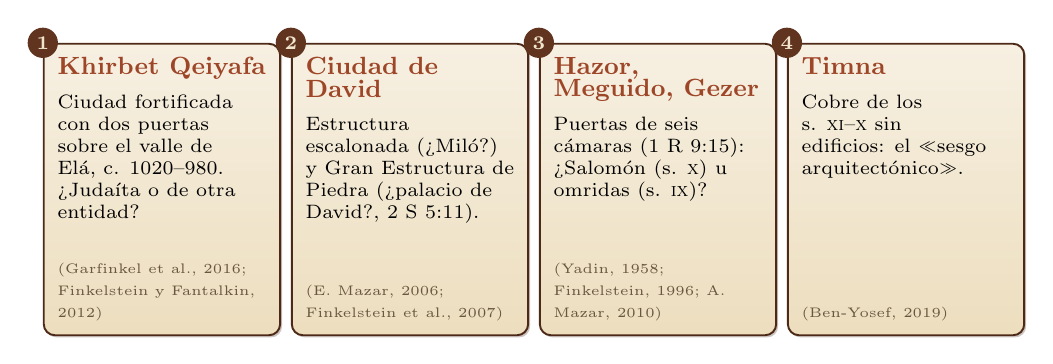
\begin{tikzpicture}
 \foreach \x/\n/\t/\d/\r in {0/1/{Khirbet Qeiyafa}/{Ciudad fortificada con dos puertas sobre el valle de Elá, c. 1020--980. ¿Judaíta o de otra entidad?}/{Garfinkel et~al., 2016; Finkelstein y Fantalkin, 2012},
   3.15/2/{Ciudad de David}/{Estructura escalonada (¿Miló?) y Gran Estructura de Piedra (¿palacio de David?, 2~S 5:11).}/{E. Mazar, 2006; Finkelstein et~al., 2007},
   6.3/3/{Hazor, Meguido, Gezer}/{Puertas de seis cámaras (1~R 9:15): ¿Salomón (s. \textsc{x}) u omridas (s. \textsc{ix})?}/{Yadin, 1958; Finkelstein, 1996; A. Mazar, 2010},
   9.45/4/{Timna}/{Cobre de los s. \textsc{xi}--\textsc{x} sin edificios: el «sesgo arquitectónico».}/{Ben-Yosef, 2019}}{
  \node[caja,anchor=north] (b\n) at (\x,0) {\parbox[t][3.35cm][t]{2.65cm}{\RaggedRight
    {\small\textbf{\textcolor{ladrillo}{\t}}}\\[4pt]\scriptsize \d\par\vfill{\tiny\color{sepia}(\r)}}};
  \node[circle,fill=cafe,text=piedra,font=\scriptsize\bfseries,inner sep=1.6pt] at (b\n.north west) {\n};}
\end{tikzpicture}\par\vspace{5pt}
\begin{minipage}{0.95\linewidth}\scriptsize \textbf{Cronología baja} (Finkelstein): David y Salomón, jefes de un reino pequeño. \textbf{Convencional modificada} (A. Mazar) y Garfinkel: un Judá organizado ya hacia el 1000. Del templo de Salomón no hay restos excavados; paralelo: Ain Dara (Monson, 2000).\end{minipage}
\end{frame}


% ===================================================
\section{David}
\begin{frame}{Hebrón: un pacto con el norte}
\begin{columns}[t,onlytextwidth]
\begin{column}{0.50\textwidth}
\centering{\large\heb{הִנְנוּ עַצְמְךָ וּבְשָׂרְךָ אֲנָחְנוּ}}\par\smallskip
\begin{cita}Henos aquí, hueso tuyo y carne tuya somos. [\ldots] Y el rey David hizo pacto con ellos en Hebrón delante de YHWH.\fuente{(2~S 5:1, 3)}\end{cita}
\small La unidad fue una unión \destacar{por pacto} (\heb{בְּרִית}): en Siquem el norte pedirá renegociarla (1~R 12:4).
\end{column}
\begin{column}{0.47\textwidth}\small
\begin{itemize}
\item \textbf{2~S 2:4}: David, rey de «la casa de Judá».
\item \textbf{2~S 2:9}: Is-boset, rey de «todo Israel» (= el norte).
\item \textbf{2~S 19:43 [19:44]}: «Diez partes tenemos nosotros en el rey».
\end{itemize}
\begin{cita}[fontupper=\scriptsize\itshape]No tenemos parte en David ni heredad en el hijo de Isaí. ¡Cada uno a sus tiendas, Israel!\fuente{(2~S 20:1; cf. 1~R 12:16)}\end{cita}
\end{column}
\end{columns}
\end{frame}

\begin{frame}{Jerusalén y el arca en Sion}
\begin{columns}[t,onlytextwidth]
\begin{column}{0.49\textwidth}\small
\begin{itemize}
\item Jebús, plaza neutral entre Judá y Benjamín (Jos 15:8; 18:16).
\item El arca sube a Sion; David danza «ceñido con un efod de lino» (2~S 6:14), ofrece y bendice en el nombre de YHWH (6:17--18).
\item Sion: el lugar que Dios «escogió» (Sal 132:13--14).
\end{itemize}
\end{column}
\begin{column}{0.49\textwidth}
\begin{cita}Desechó la tienda de José, y no escogió la tribu de Efraín, sino que escogió la tribu de Judá, el monte Sion, al cual amó [\ldots] y eligió a David su siervo.\fuente{(Sal 78:67--70)}\end{cita}
\precision{Silo, santuario de Efraín, queda atrás (Sal 78:60). Sion une y también resiente al norte.}
\end{column}
\end{columns}
\end{frame}

\begin{frame}{«Tú eres ese hombre»}
\begin{columns}[t,onlytextwidth]
\begin{column}{0.49\textwidth}\small
\begin{itemize}
\item Betsabé y Urías (2~S 11).
\item Natán: \heb{אַתָּה הָאִישׁ} (12:7). David: \heb{חָטָאתִי לַיהוָה} (12:13).
\item Perdón y consecuencia: «no se apartará jamás la espada de tu casa» (12:10).
\item Salomón: \heb{יְדִידְיָהּ}, «amado de YH» (12:25).
\item Absalón se proclama rey en Hebrón (15:10).
\end{itemize}
\end{column}
\begin{column}{0.49\textwidth}
\centering{\large\heb{לֵב טָהוֹר בְּרָא־לִי אֱלֹהִים}}\par\smallskip
\begin{cita}Crea en mí, oh Dios, un corazón limpio, y renueva un espíritu firme dentro de mí.\fuente{(Sal 51:10 [51:12])}\end{cita}
\scriptsize \heb{בָּרָא}: verbo de Gn 1:1. \heb{נָכוֹן}, «firme», como el trono de 2~S 7:16 (observación propia).\par\smallskip
\precision{la era de Arauna (2~S 24) será el monte Moriah del templo (2~Cr 3:1; cf. Gn 22).}
\end{column}
\end{columns}
\end{frame}

% ===================================================
\section{El pacto}
\begin{frame}{Una casa para David}
\fotolado{panel_2s7.jpg}{Elaboración propia: 2~S 7:13--14 en texto hebreo consonántico (BHS).}
\begin{columns}[c,onlytextwidth]
\begin{column}{0.57\textwidth}
\begin{cita}Él edificará casa a mi nombre, y yo afirmaré para siempre el trono de su reino. Yo le seré a él padre, y él me será a mí hijo [\ldots]; mi misericordia no se apartará de él.\fuente{(2~S 7:13--15)}\end{cita}
\scriptsize
\begin{itemize}
\item 7:2: David en «casa de cedro» (\emph{palacio}).
\item 7:5: «¿Tú me edificarás casa?» (\emph{templo}).
\item 7:11: «YHWH te hará casa» (\emph{dinastía}).
\item 7:16: «firme tu casa [\ldots] para siempre».
\end{itemize}
\small\destacar{David quería dar a Dios una casa; Dios le da a David una casa.}
\end{column}
\begin{column}{0.41\textwidth}\end{column}
\end{columns}
\end{frame}

\begin{frame}{Cuatro claves de 2 S 7}
\centering
\begin{tikzpicture}
 \foreach \x/\n/\t/\d/\r in {0/1/{Firme}/{\heb{נֶאְמַן} (raíz \emph{'mn}) y \heb{נָכוֹן} (raíz \emph{kun}): la promesa descansa en la fidelidad de Dios.}/{2~S 7:16; Is 55:3},
   3.15/2/{Para siempre}/{\heb{עַד־עוֹלָם}: tiempo sin límite a la vista, reforzado por el sol y la luna.}/{Sal 89:36--37 [89:37--38]},
   6.3/3/{Hijo}/{Adopción real: «yo le seré padre». Israel es también hijo (Éx 4:22).}/{Sal 2:7; Heb 1:5; 2~Co 6:18},
   9.45/4/{Disciplina}/{Castigo con «vara de hombres», pero la \emph{jésed} no se aparta.}/{2~S 7:14--15; Sal 89:30--33}}{
  \node[caja,anchor=north] (b\n) at (\x,0) {\parbox[t][3.1cm][t]{2.65cm}{\RaggedRight
    {\small\textbf{\textcolor{ladrillo}{\t}}}\\[4pt]\scriptsize \d\par\vfill{\tiny\color{sepia}(\r)}}};
  \node[circle,fill=cafe,text=piedra,font=\scriptsize\bfseries,inner sep=1.6pt] at (b\n.north west) {\n};}
\end{tikzpicture}\par\vspace{6pt}
\begin{minipage}{0.95\linewidth}\scriptsize\precision{\emph{berit} no aparece en 2~S 7, pero otros textos lo llaman pacto: «pacto perpetuo» (2~S 23:5; Sal 89:3 [89:4]; 132:12; Jer 33:21). Otros lo formulan en condicional (1~R 2:4; Sal 132:12): la promesa no depende de cada rey, pero cada rey puede perder su disfrute.}\end{minipage}
\end{frame}

\begin{frame}{«Él me será hijo»: del hebreo a Pablo}
\centering
\begin{tikzpicture}[node distance=0.9cm]
\node[caja,text width=3.3cm,align=center] (h) {\textbf{Hebreo (2~S 7:14)}\\[3pt]\heb{וְהוּא יִהְיֶה־לִּי לְבֵן}\\[2pt]el hijo de David,\\hijo de Dios};
\node[caja,text width=3.3cm,align=center,right=of h] (g) {\textbf{LXX}\\[3pt]\grc{αὐτὸς ἔσται μοι εἰς υἱόν}\\[2pt]citado en Heb 1:5};
\node[caja,text width=3.3cm,align=center,right=of g] (p) {\textbf{Pablo}\\[3pt]\grc{εἰς υἱοὺς καὶ θυγατέρας}\\[2pt]2~Co 6:18; Ro 1:3--4};
\draw[-{Latex[length=2.5mm]},oro!90!ladrillo,line width=1.4pt] (h) -- (g);
\draw[-{Latex[length=2.5mm]},oro!90!ladrillo,line width=1.4pt] (g) -- (p);
\end{tikzpicture}\par\vspace{8pt}
\scriptsize\renewcommand{\arraystretch}{1.2}
\begin{tabular}{>{\RaggedRight\arraybackslash}p{2.3cm}>{\RaggedRight\arraybackslash}p{4.0cm}>{\RaggedRight\arraybackslash}p{4.0cm}}
\toprule
& \textbf{2~S 7} & \textbf{1~Cr 17}\\\midrule
Descendiente & «que saldrá de tus entrañas» (7:12) & «uno de tus hijos» (17:11)\\
Castigo & «si hace mal, lo castigaré» (7:14) & omitido (17:13)\\
Reino & «\emph{tu} casa y \emph{tu} reino» (7:16) & «\emph{mi} casa y \emph{mi} reino» (17:14)\\
\bottomrule
\end{tabular}
\end{frame}

% ===================================================
\section{Salomón}
\begin{frame}{El templo y la gloria}
\begin{columns}[t,onlytextwidth]
\begin{column}{0.49\textwidth}\small
\begin{itemize}
\item \heb{לֵב שֹׁמֵעַ}: «un corazón que escucha» (1~R 3:9).
\item «Judá e Israel eran muchos, como la arena del mar» (1~R 4:20; Gn 22:17).
\item Templo: 480 años tras el Éxodo (1~R 6:1); planta tripartita.
\item Columnas \heb{יָכִין} (\emph{Yajín}, «él establecerá», raíz \emph{kun}) y \heb{בֹּעַז} (7:21).
\item Dedicación en Sucot, «el mes séptimo» (8:2).
\end{itemize}
\end{column}
\begin{column}{0.49\textwidth}
\begin{cita}La nube llenó la casa de YHWH, y los sacerdotes no pudieron permanecer para ministrar [\ldots], porque la gloria de YHWH había llenado la casa.\fuente{(1~R 8:10--11)}\end{cita}
\begin{cita}[fontupper=\scriptsize\itshape]Los cielos de los cielos no te pueden contener; ¡cuánto menos esta casa!\fuente{(1~R 8:27)}\end{cita}
\end{column}
\end{columns}
\end{frame}

\begin{frame}{Una oración que prevé el exilio}
\centering{\large\heb{וְהֵשִׁיבוּ אֶל־לִבָּם בָּאָרֶץ אֲשֶׁר נִשְׁבּוּ־שָׁם וְשָׁבוּ}}\par\smallskip
\begin{cita}Si pecaren contra ti, porque no hay hombre que no peque, [\ldots] y ellos volvieren en sí en la tierra adonde fueron llevados cautivos, y se convirtieren y oraren a ti [\ldots] con el rostro hacia su tierra, [\ldots] tú oirás en los cielos [\ldots] y les harás hallar misericordia.\fuente{(1~R 8:46--48, 50)}\end{cita}
\begin{columns}[t,onlytextwidth]
\begin{column}{0.49\textwidth}\small
\heb{שׁוּב} (\emph{shuv}, volver) y \heb{שָׁבָה} (\emph{shavá}, llevar cautivo): el regreso del corazón precede al regreso a la tierra (Dt 30:1--5).
\end{column}
\begin{column}{0.49\textwidth}\small
Siete súplicas (8:31--53); ya la segunda pide: «vuélvelos a la tierra» (8:34). En su máxima gloria, Israel ora por su exilio.
\end{column}
\end{columns}
\end{frame}

\begin{frame}{Nación santa: vivida, quebrada, preservada}
\begin{columns}[t,onlytextwidth]
\begin{column}{0.32\textwidth}\scriptsize
\textbf{\textcolor{ladrillo}{Vivida}}\par\smallskip
David con efod, ofrece y bendice (2~S 6:14--18). «Sacerdote [\ldots] según Melquisedec» (Sal 110:4). Salomón ora por el extranjero: «que todos los pueblos conozcan tu nombre» (1~R 8:41--43). La reina de Sabá bendice a YHWH (1~R 10:9; Is 60:6). «Benditas serán en él todas las naciones» (Sal 72:17; Gn 12:3).
\end{column}
\begin{column}{0.33\textwidth}\scriptsize
\textbf{\textcolor{ladrillo}{Quebrada}}\par\smallskip
El rey hace del pueblo un Egipto (\emph{mas}). El que oró por las naciones levanta altares a sus dioses (1~R 11:7). Jeroboam separa el sacerdocio de la elección (1~R 12:31).
\end{column}
\begin{column}{0.32\textwidth}\scriptsize
\textbf{\textcolor{ladrillo}{Preservada}}\par\smallskip
Profetas sobre el rey: Natán, Gad, Ahías, Semaías. Arrepentimiento (Sal 51; 1~R 8:47). Remanente en ambos reinos: levitas en Judá (2~Cr 11) y los siete mil del norte (1~R 19:18; Ro 11:4).
\end{column}
\end{columns}\par\vspace{8pt}
\begin{tcolorbox}[colback=piedra,colframe=cafe,boxrule=0.8pt,arc=3pt,fontupper=\small]
«Mi casa será llamada casa de oración para todos los pueblos» (Is 56:7).
\end{tcolorbox}
\end{frame}

% ===================================================
\section{La división}
\begin{frame}{Cuatro causas de la división}
\centering
\begin{tikzpicture}
 \foreach \x/\n/\t/\d/\r in {0/1/{Idolatría}/{Altares a Quemos y Moloc frente a Jerusalén; «sus mujeres desviaron su corazón».}/{1~R 11:1--13},
   3.15/2/{Trabajo forzado}/{\heb{מַס} (\emph{mas}) sobre «todo Israel»; Jeroboam, sobre «la casa de José».}/{1~R 5:13 [5:27]; 11:28},
   6.3/3/{Profecía}/{Ahías de Silo rasga el manto en doce pedazos.}/{1~R 11:29--39},
   9.45/4/{Necedad}/{Roboam en Siquem: «yo os castigaré con escorpiones».}/{1~R 12:1--15}}{
  \node[caja,anchor=north] (b\n) at (\x,0) {\parbox[t][3.0cm][t]{2.65cm}{\RaggedRight
    {\small\textbf{\textcolor{ladrillo}{\t}}}\\[4pt]\scriptsize \d\par\vfill{\tiny\color{sepia}(\r)}}};
  \node[circle,fill=cafe,text=piedra,font=\scriptsize\bfseries,inner sep=1.6pt] at (b\n.north west) {\n};}
\end{tikzpicture}\par\vspace{6pt}
\begin{minipage}{0.95\linewidth}\small Detrás de todo, la ley del rey violada: caballos de Egipto, mujeres, oro (Dt 17:16--17; 1~R 10:14, 26--29; 11:3). Y una tensión norte--sur anterior a Salomón (2~S 19--20).\par\smallskip
\destacar{El rey se hace faraón}: \emph{mas} es la palabra de Éx 1:11 (\heb{שָׂרֵי מִסִּים}); «tu padre agravó nuestro yugo» (1~R 12:4).\par
\precision{1~R 9:20--22 reserva la servidumbre permanente a los cananeos; a los israelitas, una leva por turnos (Cogan, 2001).}\end{minipage}
\end{frame}


\begin{frame}{Diez pedazos para Jeroboam}
\fotolado{panel_1r11.jpg}{Elaboración propia: 1~R 11:39 en texto hebreo consonántico (BHS).}
\begin{columns}[c,onlytextwidth]
\begin{column}{0.57\textwidth}
\begin{cita}A ti te daré diez tribus; y él tendrá una tribu por amor a David mi siervo, y por amor a Jerusalén [\ldots], para que mi siervo David tenga lámpara todos los días delante de mí.\fuente{(1~R 11:31--32, 36)}\end{cita}
\begin{cita}Y yo afligiré a la descendencia de David a causa de esto, \textbf{pero no para siempre}.\fuente{(1~R 11:39)}\end{cita}
\scriptsize \heb{אַךְ לֹא כָל־הַיָּמִים}: «pero no todos los días». \heb{נִיר}, «lámpara»: la continuidad de la casa de David.\par\smallskip
\precision{10 + 1 no son 12: ¿Benjamín, Simeón absorbido, Leví sin territorio? (1~R 12:21).}
\end{column}
\begin{column}{0.41\textwidth}\end{column}
\end{columns}
\end{frame}

\begin{frame}{Siquem: «¡A tus tiendas, Israel!»}
\centering{\large\heb{מַה־לָּנוּ חֵלֶק בְּדָוִד}}\par\smallskip
\begin{cita}¿Qué parte tenemos nosotros con David? No tenemos heredad en el hijo de Isaí. ¡Israel, a tus tiendas! ¡Provee ahora en tu casa, David!\fuente{(1~R 12:16)}\end{cita}
\begin{columns}[t,onlytextwidth]
\begin{column}{0.49\textwidth}\small
\begin{itemize}
\item Coronación en Siquem, lugar del pacto (Jos 24): el norte renegocia.
\item «La causa venía de YHWH» (12:15).
\item «Tu casa, David»: la palabra de 2~S 7, ahora como rechazo.
\end{itemize}
\end{column}
\begin{column}{0.49\textwidth}\small
\begin{itemize}
\item «Todo Israel» (= el norte) hace rey a Jeroboam (12:20).
\item Judá y Benjamín siguen a David (12:21).
\item Semaías: «no peleéis contra vuestros \textbf{hermanos}» (12:24).
\end{itemize}
\end{column}
\end{columns}
\end{frame}

\begin{frame}{Los becerros de Betel y Dan}
\begin{columns}[t,onlytextwidth]
\begin{column}{0.50\textwidth}
\centering{\small\heb{הִנֵּה אֱלֹהֶיךָ יִשְׂרָאֵל}}\par\smallskip
\begin{cita}He aquí tus dioses, oh Israel, los cuales te hicieron subir de la tierra de Egipto.\fuente{(1~R 12:28; cf. Éx 32:4)}\end{cita}
\scriptsize
\begin{itemize}
\item El norte nace repitiendo el pecado del Sinaí.
\item Sacerdotes no levitas; fiesta del mes octavo, copia de Sucot «inventada de su corazón» (12:31--33).
\end{itemize}
\end{column}
\begin{column}{0.47\textwidth}\small
\textbf{\textcolor{cafe}{Respuesta: migración al sur}}\par\smallskip
Sacerdotes, levitas y fieles «de todas las tribus de Israel» se van a Judá (2~Cr 11:13--17); siguen bajo Asa (2~Cr 15:9) y Ezequías (2~Cr 30).\par\medskip
\precision{¿ídolos o pedestales de YHWH invisible, como los querubines? El narrador lo llama «el pecado de Jeroboam» (1~R 15:30).}
\end{column}
\end{columns}
\end{frame}


% ===================================================
\section{Tradición judía}
\begin{frame}{El renuevo de David en la Amidá}
\centering{\large\heb{אֶת צֶמַח דָּוִד עַבְדְּךָ מְהֵרָה תַצְמִיחַ}}\par\smallskip
\begin{cita}Haz brotar pronto el renuevo de David tu siervo, y exalta su poder con tu salvación, porque tu salvación esperamos todo el día.\fuente{(Amidá, bendición 15)}\end{cita}
\begin{columns}[t,onlytextwidth]
\begin{column}{0.49\textwidth}\small
\textbf{\textcolor{cafe}{Origen bíblico}}: \emph{tsémaj} (Jer 23:5; 33:15); «haré brotar el poder de David» (Sal 132:17). Bendición 14: «el trono de David establece pronto» en Jerusalén.
\end{column}
\begin{column}{0.49\textwidth}\small
\textbf{\textcolor{cafe}{Birkat ha-Mazón}}: «sobre el reino de la casa de David tu ungido» (atribuida a David y Salomón, Berajot 48b). En Sucot: «levante la cabaña caída de David» (Am 9:11).
\end{column}
\end{columns}
\end{frame}

\begin{frame}{David y Jeroboam en el Talmud}
\begin{columns}[t,onlytextwidth]
\begin{column}{0.49\textwidth}\scriptsize
\begin{itemize}
\item \textbf{El arpa}: el viento del norte despertaba a David a medianoche (Berajot 3b).
\item \textbf{El pecado}: «para enseñar el arrepentimiento al individuo» (Avodá Zará 4b--5a); otra opinión niega que pecara (Shabat 56a).
\item «David, rey de Israel, vive y permanece» (Rosh Hashaná 25a); «otro David» (Sanedrín 98b).
\item \textbf{Jeroboam}: sin parte en el mundo venidero (Mishná, Sanedrín 10:2). «¿Quién irá delante?» «El hijo de Isaí». «Entonces no quiero» (Sanedrín 102a).
\end{itemize}
\end{column}
\begin{column}{0.49\textwidth}\scriptsize
\textbf{\textcolor{cafe}{Jerusalén en el rito}}: orar hacia la tierra, la ciudad, el templo y el santísimo (Berajot 30a; 1~R 8:44, 48). Confesión de Yom Kipur discutida desde 1~R 8:47 (Yomá 36b). Tisha be-Av: caída de los dos templos (Mishná, Taanit 4:6).\par\medskip
\textbf{\textcolor{cafe}{Antes del NT}}: 4Q174 aplica 2~S 7 al «Renuevo de David» (\heb{צמח דויד}); \emph{Sal. Salom.} 17:21, «el hijo de David»; Targum de Is 11:1, «el Mesías». Josefo, \emph{Ant.} 7--8.
\end{column}
\end{columns}
\end{frame}

% ===================================================
\section{Restauración}
\begin{frame}{El límite del juicio}
\centering\scriptsize\renewcommand{\arraystretch}{1.25}
\begin{tabular}{>{\RaggedRight\arraybackslash}p{1.9cm}>{\RaggedRight\arraybackslash}p{4.6cm}>{\RaggedRight\arraybackslash}p{4.4cm}}
\toprule
\textbf{Texto} & \textbf{Promesa} & \textbf{Proyección}\\\midrule
2~S 7:14--16 & La \emph{jésed} no se aparta; trono «para siempre» & Is 55:3; Lc 1:32--33\\
Sal 132:11, 17 & Juramento; renuevo y lámpara & Jer 23:5; Hch 2:30\\
1~R 8:46--53 & Regreso del corazón y de la tierra & Dt 30:1--5; Dn 9:4--19\\
1~R 11:36, 39 & Lámpara; afligir «pero no para siempre» & Am 9:11; Os 3:5; Ez 37:22--25\\
\bottomrule
\end{tabular}\par\vspace{6pt}
\begin{cita}Señor, ¿dónde están tus antiguas misericordias, que juraste a David por tu fidelidad?\fuente{(Sal 89:49 [89:50])}\end{cita}
{\small\itshape\color{sepia}El Sal 89 no resuelve la tensión entre promesa y corona caída: la lleva a Dios.}
\end{frame}

\begin{frame}{Isaías: el tronco de Isaí}
\begin{columns}[t,onlytextwidth]
\begin{column}{0.50\textwidth}
\centering{\heb{וְיָצָא חֹטֶר מִגֵּזַע יִשָׁי}}\par\smallskip
\begin{cita}Saldrá una vara del tronco de Isaí [\ldots]. La raíz de Isaí, puesta por pendón a los pueblos, será buscada por las naciones.\fuente{(Is 11:1, 10)}\end{cita}
\scriptsize \heb{גֵּזַע}, «tocón»: el árbol ha sido cortado. Pablo: Ro 15:12 (LXX, \grc{ὁ ἀνιστάμενος}).
\end{column}
\begin{column}{0.47\textwidth}
\begin{cita}[fontupper=\scriptsize\itshape]Juntará los desterrados de Israel, y reunirá los esparcidos de Judá [\ldots]. Efraín no tendrá envidia de Judá, ni Judá afligirá a Efraín.\fuente{(Is 11:12--13)}\end{cita}
\scriptsize
\begin{itemize}
\item Is 9:6--7 [9:5--6]: el niño en el trono de David; luz primero sobre Galilea, el norte deportado.
\item Is 55:3: «las misericordias firmes de David» (Hch 13:34).
\end{itemize}
\end{column}
\end{columns}
\end{frame}

\begin{frame}{Jeremías: el renuevo justo}
\begin{columns}[t,onlytextwidth]
\begin{column}{0.50\textwidth}
\centering{\heb{וַהֲקִמֹתִי לְדָוִד צֶמַח צַדִּיק}}\par\smallskip
\begin{cita}Levantaré a David renuevo justo [\ldots]. En sus días será salvo \textbf{Judá}, e \textbf{Israel} habitará confiado; y este será su nombre: YHWH, justicia nuestra.\fuente{(Jer 23:5--6)}\end{cita}
\end{column}
\begin{column}{0.47\textwidth}\small
\begin{itemize}
\item Salva a los dos reinos.
\item \emph{YHWH tsidqenu} frente a Sedequías (\emph{Tsidqiyahu}).
\item Jer 33:20--21: pacto con David como el pacto con el día y la noche.
\item Jer 33:24--26: «las dos familias» no serán desechadas.
\end{itemize}
\precision{Jer 33:14--26 falta en la LXX; se sigue el TM.}
\end{column}
\end{columns}
\end{frame}

\begin{frame}{Ezequiel: dos palos}
\fotolado{panel_ez37.jpg}{Elaboración propia: Ez 37:22 en texto hebreo consonántico (BHS).}
\begin{columns}[c,onlytextwidth]
\begin{column}{0.57\textwidth}
\begin{cita}Los haré una nación en la tierra, en los montes de Israel, y un rey será a todos ellos por rey; y nunca más serán dos naciones, ni nunca más serán divididos en dos reinos. [\ldots] Mi siervo David será rey sobre ellos.\fuente{(Ez 37:22, 24)}\end{cita}
\scriptsize
\begin{itemize}
\item Un palo «para Judá», otro «para José, palo de Efraín» (37:16).
\item Deshace 1~R 12: dos reinos $\to$ una nación; dos reyes $\to$ un rey, «David».
\item Pacto perpetuo y santuario en medio de ellos (37:26--28).
\end{itemize}
\end{column}
\begin{column}{0.41\textwidth}\end{column}
\end{columns}
\end{frame}

\begin{frame}{Amós y Oseas}
\begin{columns}[t,onlytextwidth]
\begin{column}{0.49\textwidth}
\textbf{\textcolor{cafe}{Amós, en Betel}}
\begin{cita}[fontupper=\scriptsize\itshape]En aquel día yo levantaré la cabaña caída de David [\ldots], para que posean el resto de Edom y todas las naciones sobre las cuales es invocado mi nombre.\fuente{(Am 9:11--12)}\end{cita}
\scriptsize Jacobo lo cita en Hch 15:16--17 según la LXX: «para que el resto de los hombres busque al Señor».\par
\precision{TM \emph{yirshú} / \emph{Edom}; LXX «busquen» / «hombres» (\emph{adam}).}
\end{column}
\begin{column}{0.49\textwidth}
\textbf{\textcolor{cafe}{Oseas, profeta del norte}}
\begin{cita}[fontupper=\scriptsize\itshape]Después volverán los hijos de Israel, y buscarán a YHWH su Dios, y a David su rey.\fuente{(Os 3:5)}\end{cita}
\scriptsize El norte volverá a la casa que rechazó en Siquem. «Se congregarán los hijos de Judá y de Israel, y nombrarán un solo jefe» (Os 1:11 [2:2]). ONE FOR ISRAEL (2025) cita Os 3:4--5.
\end{column}
\end{columns}
\end{frame}

\begin{frame}{Lucas y Pablo: el hijo de David}
\fotolado{panel_lc1.jpg}{Elaboración propia: Lc 1:32--33 en escritura uncial (texto NA28).}
\begin{columns}[c,onlytextwidth]
\begin{column}{0.57\textwidth}
\begin{cita}El Señor Dios le dará el trono de David su padre; y reinará sobre la casa de Jacob para siempre.\fuente{(Lc 1:32--33)}\end{cita}
\scriptsize
\begin{itemize}
\item \textbf{Ro 1:3--4}: \grc{ἐκ σπέρματος Δαυὶδ κατὰ σάρκα}, declarado Hijo de Dios por la resurrección (2~S 7:12--14).
\item \textbf{Ro 15:12}: la raíz de Isaí; las naciones esperarán en él.
\item \textbf{Ro 11:1--4}: «¿Ha desechado Dios a su pueblo?» Pablo, benjaminita; Elías, ejemplo del norte.
\item \textbf{Ro 11:26}: «Vendrá de \textbf{Sion} el Libertador».
\end{itemize}
\precision{2~Ti 2:8 dice lo mismo; su autoría se discute, pero Ro 1:3--4 basta.}
\end{column}
\begin{column}{0.41\textwidth}\end{column}
\end{columns}
\end{frame}

% ===================================================
\section{Síntesis}
\begin{frame}{Síntesis}
\begin{tcolorbox}[colback=piedra,colframe=ladrillo,boxrule=1pt,arc=3pt,fontupper=\small]
\textbf{\textcolor{cafe}{Israel de David a la división:}} un pueblo unido por pacto bajo un rey al que Dios prometió una casa «para siempre», con un templo para todas las naciones; un reino partido por la idolatría y la opresión, pero bajo un juicio con límite: «no para siempre» (1~R 11:39). Los profetas esperan un hijo de David bajo el cual Efraín y Judá vuelvan a ser una nación (Ez 37:22).
\end{tcolorbox}
\scriptsize\renewcommand{\arraystretch}{1.2}
\begin{tabular}{>{\RaggedRight\arraybackslash}p{3.0cm}>{\RaggedRight\arraybackslash}p{8.3cm}}
\toprule
\textbf{Eje} & \textbf{Lo que deja esta etapa}\\\midrule
Unidad frágil & Pacto de Hebrón; tensión norte--sur (2~S 5:3; 19:41--20:1)\\
Vocación & Arca en Sion; templo para los pueblos; Sal 72:17\\
Restauración & 2~S 7:14--16; 1~R 8:46--53; 11:36--39; Sal 89\\
Proyección & Is 11; Jer 23; Ez 37; Am 9; Os 3:5; Ro 1:3--4; 11:1, 26\\
\bottomrule
\end{tabular}
\end{frame}

\begin{frame}{¿Cómo volverán a ser uno?}
\begin{columns}[c,onlytextwidth]
\begin{column}{0.55\textwidth}
\begin{cita}Júntalos luego el uno con el otro, para que sean uno solo, y serán uno solo en tu mano.\fuente{(Ez 37:17)}\end{cita}
\small Antes de esa respuesta, los dos reinos recorrerán caminos distintos: \destacar{Israel (norte)}, con capital en Samaria, cae ante Asiria (722 a.\,e.\,c.); \destacar{Judá}, con la casa de David, cae ante Babilonia (586 a.\,e.\,c.) y vuelve.
\end{column}
\begin{column}{0.42\textwidth}
\begin{tcolorbox}[colback=cafe,colframe=cafeosc,coltext=piedra,boxrule=0.8pt,arc=3pt,fontupper=\small]
\textbf{Estudio 5}\par\smallskip
Los reyes y los cautiverios: reino dividido, Asiria y Babilonia, profetas y promesas de nuevo pacto y reunificación (Jer 31; Ez 36--37).
\end{tcolorbox}
\end{column}
\end{columns}
\end{frame}

\begin{frame}{Para la reflexión}
\small
\begin{enumerate}
\item David quiso construir una casa para Dios, y Dios le prometió una casa a él (2~S 7:5, 11). ¿Qué dice ese giro sobre cómo Dios cumple su propósito?
\item ¿Cómo se sostiene una promesa «para siempre» cuando los hechos parecen negarla (Sal 89)?
\item Salomón oró por el extranjero y levantó altares a dioses extranjeros. ¿Qué enseña esa contradicción?
\item ¿Qué parte de la división fue responsabilidad de Judá y qué parte de Israel (norte)?
\item Pablo, benjaminita, toma su ejemplo de remanente del reino del norte (Ro 11:1--4). ¿Qué sugiere sobre «todo Israel»?
\end{enumerate}
\end{frame}

\begin{frame}{Glosario}
\begin{columns}[t,onlytextwidth]
\begin{column}{0.49\textwidth}\scriptsize
\textbf{Ad olam} (\heb{עַד־עוֹלָם}): «para siempre» (2~S 7:16).\par\smallskip
\textbf{Báyit} (\heb{בַּיִת}): casa: palacio, templo, dinastía.\par\smallskip
\textbf{Bet David} (\heb{בֵּית דָּוִד}): casa de David; \emph{bytdwd} en Tel Dan.\par\smallskip
\textbf{Efraín} (\heb{אֶפְרַיִם}): tribu central; nombre del reino del norte.\par\smallskip
\textbf{Jésed} (\heb{חֶסֶד}): misericordia leal al pacto.\par\smallskip
\textbf{Kun} (\heb{כּוּן}): establecer; \emph{najón}, \emph{Yajín}.
\end{column}
\begin{column}{0.49\textwidth}\scriptsize
\textbf{Mas} (\heb{מַס}): leva de trabajo forzado (Éx 1:11; 1~R 5:13).\par\smallskip
\textbf{Mashíaj} (\heb{מָשִׁיחַ}): ungido; \grc{Χριστός}.\par\smallskip
\textbf{Nir} (\heb{נִיר}): lámpara de David (1~R 11:36).\par\smallskip
\textbf{Shuv} (\heb{שׁוּב}): volver, convertirse (1~R 8:47).\par\smallskip
\textbf{Sukkat David} (\heb{סֻכַּת דָּוִיד}): cabaña de David (Am 9:11).\par\smallskip
\textbf{Tsémaj} (\heb{צֶמַח}): renuevo (Jer 23:5; Amidá 15).
\end{column}
\end{columns}
\end{frame}

\begin{frame}{Referencias}
\begin{columns}[t,onlytextwidth]
\begin{column}{0.49\textwidth}\fontsize{4.6}{5.4}\selectfont
\refapa{Alter, R. (1999). \emph{The David story}. W.~W. Norton.}
\refapa{Ben-Yosef, E. (2019). The architectural bias in current biblical archaeology. \emph{Vetus Testamentum, 69}(3), 361--387.}
\refapa{\emph{Biblia Hebraica Stuttgartensia} (5.ª ed.). (1997). Deutsche Bibelgesellschaft.}
\refapa{Biran, A., \& Naveh, J. (1993). An Aramaic stele fragment from Tel Dan. \emph{Israel Exploration Journal, 43}(2--3), 81--98.}
\refapa{Biran, A., \& Naveh, J. (1995). The Tel Dan inscription: A new fragment. \emph{Israel Exploration Journal, 45}(1), 1--18.}
\refapa{Broshi, M., \& Finkelstein, I. (1992). The population of Palestine in Iron Age II. \emph{BASOR, 287}, 47--60.}
\refapa{Charlesworth, J.~H. (Ed.). (1983--1985). \emph{The Old Testament pseudepigrapha}. Doubleday.}
\refapa{Chilton, B.~D. (1987). \emph{The Isaiah Targum}. Michael Glazier.}
\refapa{Cogan, M. (2001). \emph{1 Kings} (Anchor Bible 10). Doubleday.}
\refapa{Departamento de Educación, Congregación Iglesia Israelita del Nuevo Pacto. (s.\,f.). \emph{Restauración de Israel} (Clase 7) [Presentación].}
\refapa{Elbogen, I. (1993). \emph{Jewish liturgy: A comprehensive history}. Jewish Publication Society.}
\refapa{Epstein, I. (Ed.). (1935--1948). \emph{The Babylonian Talmud}. Soncino Press.}
\refapa{Finkelstein, I. (1996). The archaeology of the United Monarchy: An alternative view. \emph{Levant, 28}, 177--187.}
\refapa{Finkelstein, I., \& Fantalkin, A. (2012). Khirbet Qeiyafa: An unsensational archaeological and historical interpretation. \emph{Tel Aviv, 39}(1), 38--63.}
\refapa{Finkelstein, I., Herzog, Z., Singer-Avitz, L., \& Ussishkin, D. (2007). Has King David's palace in Jerusalem been found? \emph{Tel Aviv, 34}(2), 142--164.}
\refapa{Finkelstein, I., Na'aman, N., \& Römer, T. (2019). Restoring line 31 in the Mesha Stele. \emph{Tel Aviv, 46}(1), 3--11.}
\refapa{Finkelstein, I., \& Silberman, N.~A. (2001). \emph{The Bible unearthed}. Free Press.}
\refapa{Finkelstein, I., \& Silberman, N.~A. (2006). \emph{David and Solomon}. Free Press.}
\refapa{Garfinkel, Y., Kreimerman, I., \& Zilberg, P. (2016). \emph{Debating Khirbet Qeiyafa}. Israel Exploration Society.}
\end{column}
\begin{column}{0.49\textwidth}\fontsize{4.6}{5.4}\selectfont
\refapa{Hays, R.~B. (1989). \emph{Echoes of Scripture in the letters of Paul}. Yale University Press.}
\refapa{Josefo, F. (1987). \emph{The works of Josephus} (W. Whiston, Trad.). Hendrickson.}
\refapa{Kitchen, K.~A. (1986). \emph{The Third Intermediate Period in Egypt} (2.ª ed.). Aris \& Phillips.}
\refapa{Kitchen, K.~A. (2003). \emph{On the reliability of the Old Testament}. Eerdmans.}
\refapa{Lemaire, A. (1994). «House of David» restored in Moabite inscription. \emph{Biblical Archaeology Review, 20}(3), 30--37.}
\refapa{Mazar, A. (2010). Archaeology and the biblical narrative: The case of the United Monarchy. En R.~G. Kratz \& H. Spieckermann (Eds.), \emph{One God -- one cult -- one nation}. De Gruyter.}
\refapa{Mazar, E. (2006). Did I find King David's palace? \emph{Biblical Archaeology Review, 32}(1).}
\refapa{McCarter, P.~K. (1984). \emph{II Samuel} (Anchor Bible 9). Doubleday.}
\refapa{Mendenhall, G.~E. (1958). The census lists of Numbers 1 and 26. \emph{Journal of Biblical Literature, 77}(1), 52--66.}
\refapa{Monson, J. (2000). The new \textquoteleft Ain Dara temple: Closest Solomonic parallel. \emph{Biblical Archaeology Review, 26}(3).}
\refapa{\emph{Novum Testamentum Graece} (28.ª ed.). (2012). Deutsche Bibelgesellschaft.}
\refapa{ONE FOR ISRAEL Ministry. (2025, 3 de julio). \emph{What does «all Israel will be saved» mean in Romans 11?} \url{https://www.oneforisrael.org/what-does-all-israel-will-be-saved-mean-in-romans-11/}}
\refapa{Rahlfs, A., \& Hanhart, R. (Eds.). (2006). \emph{Septuaginta} (ed. rev.). Deutsche Bibelgesellschaft.}
\refapa{Reich, R., \& Shukron, E. (1999). Light at the end of the tunnel. \emph{Biblical Archaeology Review, 25}(1).}
\refapa{Sacks, J. (Trad.). (2009). \emph{The Koren Siddur}. Koren Publishers.}
\refapa{Thiele, E.~R. (1983). \emph{The mysterious numbers of the Hebrew kings} (ed. rev.). Zondervan.}
\refapa{Vermes, G. (2004). \emph{The complete Dead Sea Scrolls in English} (ed. rev.). Penguin.}
\refapa{Wright, N.~T. (2013). \emph{Paul and the faithfulness of God}. Fortress Press.}
\refapa{Yadin, Y. (1958). Solomon's city wall and gate at Gezer. \emph{Israel Exploration Journal, 8}(2), 80--86.}
\end{column}
\end{columns}
\end{frame}
\end{document}
